\let\negmedspace\undefined
\let\negthickspace\undefined
\documentclass[journal]{IEEEtran}
\usepackage[a5paper, margin=10mm, onecolumn]{geometry}
\usepackage{lmodern}
\usepackage{tfrupee}

\setlength{\headheight}{1cm}
\setlength{\headsep}{0mm}

\usepackage{gvv-book}
\usepackage{gvv}
\usepackage{cite}
\usepackage{amsmath,amssymb,amsfonts,amsthm}
\usepackage{algorithmic}
\usepackage{graphicx}
\usepackage{textcomp}
\usepackage{xcolor}
\usepackage{txfonts}
\usepackage{listings}
\usepackage{enumitem}
\usepackage{mathtools}
\usepackage{gensymb}
\usepackage{comment}
\usepackage[breaklinks=true]{hyperref}
\usepackage{tkz-euclide} 
\usepackage{listings}                                      
\def\inputGnumericTable{}                                 
\usepackage[latin1]{inputenc}                                
\usepackage{color}                                            
\usepackage{array}                                            
\usepackage{longtable}
\usepackage{multicol}
\usepackage{calc}                                             
\usepackage{multirow}                                         
\usepackage{hhline}                                           
\usepackage{ifthen}                                           
\usepackage{lscape}

\begin{document}

\bibliographystyle{IEEEtran}
\vspace{3cm}

\title{12.8.3.9}
\author{EE24BTECH11011 - Pranay kumar}
{\let\newpage\relax\maketitle}

\renewcommand{\thefigure}{\theenumi}
\renewcommand{\thetable}{\theenumi}
\setlength{\intextsep}{10pt}

\numberwithin{equation}{enumi}
\numberwithin{figure}{enumi}
\renewcommand{\thetable}{\theenumi}

\textbf{Question}:\newline
Find the area of the smaller region bounded by the ellipse $\frac{x^2}{a^2}+\frac{y^2}{b^2}=1$ and the line $\frac{x}{a}+\frac{y}{b}=1$
\newline

\section*{Theoretical Solution}
The equation of the ellipse is 
\begin{align}
\frac{x^2}{a^2} + \frac{y^2}{b^2} = 1
\end{align}
and the line is 
\begin{align}
\frac{x}{a} + \frac{y}{b} = 1.
\end{align}
The intersection points of the ellipse and line are calculated by solving these equations simultaneously. Substituting $y = b\brak{1 - \frac{x}{a}}$ into the ellipse equation:
\begin{align}
\frac{x^2}{a^2} + \frac{\left(b\left(1 - \frac{x}{a}\right)\right)^2}{b^2} = 1.
\end{align}
Expanding and simplifying gives the roots:
\begin{align}
x_1 = 0, x_2 = a.
\end{align}
The area of the smaller region is calculated as:
\begin{align}
    A = \int_{0}^{a} \brak{b\sqrt{1 - \frac{x^2}{a^2}} - b\brak{1 - \frac{x}{a} dx.
\end{align}
Solving this integral gives:
\begin{align}
A = \frac{ab}{2} \brak{\frac{\pi}{2} - 1}.
\end{align}

\section*{Computational Solution}
The area is also calculated using the trapezoidal rule. Let $f_{\text{ellipse}}(x)$ and $f_{\text{line}}(x)$ be the equations of the ellipse and line respectively:
\begin{align}
f_{\text{ellipse}}(x) = b\sqrt{1 - \frac{x^2}{a^2}}, \quad f_{\text{line}}(x) = b\brak{1 - \frac{x}{a}}.
\end{align}
The area is computed as:
\begin{align}
A = \int_{0}^{a} \left(f_{\text{ellipse}}(x) - f_{\text{line}}(x)\right) dx.
\end{align}
Using the trapezoidal rule with $n$ intervals, the computational area is found to be:
\begin{align}
A \approx \frac{ab}{2} \brak{\frac{\pi}{2} - 1}.
\end{align}

\section*{Results}
Theoretical area: $\frac{ab}{2}\brak{\frac{\pi}{2} - 1}$ \\
Computational area: $\frac{ab}{2}\brak{\frac{\pi}{2} - 1}$

\begin{figure}[h!]
   \centering
   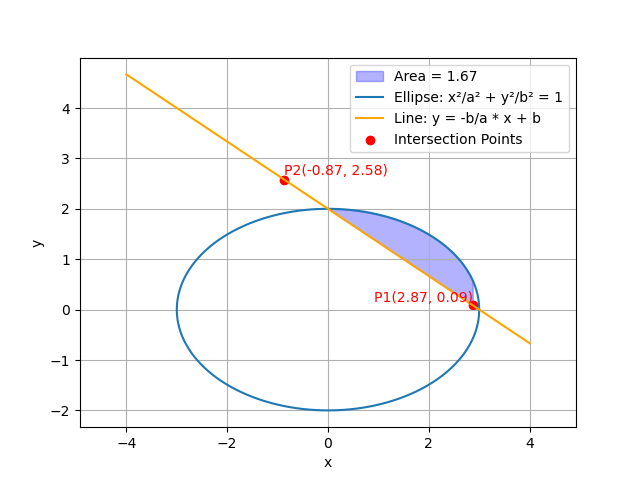
\includegraphics[width=1\linewidth]{figs/fig.png}
  
   \label{stemplot}
\end{figure}

\end{document}

